\documentclass[1p]{elsarticle_modified}
%\bibliographystyle{elsarticle-num}

%\usepackage[colorlinks]{hyperref}
%\usepackage{abbrmath_seonhwa} %\Abb, \Ascr, \Acal ,\Abf, \Afrak
\usepackage{amsfonts}
\usepackage{amssymb}
\usepackage{amsmath}
\usepackage{amsthm}
\usepackage{scalefnt}
\usepackage{amsbsy}
\usepackage{kotex}
\usepackage{caption}
\usepackage{subfig}
\usepackage{color}
\usepackage{graphicx}
\usepackage{xcolor} %% white, black, red, green, blue, cyan, magenta, yellow
\usepackage{float}
\usepackage{setspace}
\usepackage{hyperref}

\usepackage{tikz}
\usetikzlibrary{arrows}

\usepackage{multirow}
\usepackage{array} % fixed length table
\usepackage{hhline}

%%%%%%%%%%%%%%%%%%%%%
\makeatletter
\renewcommand*\env@matrix[1][\arraystretch]{%
	\edef\arraystretch{#1}%
	\hskip -\arraycolsep
	\let\@ifnextchar\new@ifnextchar
	\array{*\c@MaxMatrixCols c}}
\makeatother %https://tex.stackexchange.com/questions/14071/how-can-i-increase-the-line-spacing-in-a-matrix
%%%%%%%%%%%%%%%

\usepackage[normalem]{ulem}

\newcommand{\msout}[1]{\ifmmode\text{\sout{\ensuremath{#1}}}\else\sout{#1}\fi}
%SOURCE: \msout is \stkout macro in https://tex.stackexchange.com/questions/20609/strikeout-in-math-mode

\newcommand{\cancel}[1]{
	\ifmmode
	{\color{red}\msout{#1}}
	\else
	{\color{red}\sout{#1}}
	\fi
}

\newcommand{\add}[1]{
	{\color{blue}\uwave{#1}}
}

\newcommand{\replace}[2]{
	\ifmmode
	{\color{red}\msout{#1}}{\color{blue}\uwave{#2}}
	\else
	{\color{red}\sout{#1}}{\color{blue}\uwave{#2}}
	\fi
}

\newcommand{\Sol}{\mathcal{S}} %segment
\newcommand{\D}{D} %diagram
\newcommand{\A}{\mathcal{A}} %arc


%%%%%%%%%%%%%%%%%%%%%%%%%%%%%5 test

\def\sl{\operatorname{\textup{SL}}(2,\Cbb)}
\def\psl{\operatorname{\textup{PSL}}(2,\Cbb)}
\def\quan{\mkern 1mu \triangleright \mkern 1mu}

\theoremstyle{definition}
\newtheorem{thm}{Theorem}[section]
\newtheorem{prop}[thm]{Proposition}
\newtheorem{lem}[thm]{Lemma}
\newtheorem{ques}[thm]{Question}
\newtheorem{cor}[thm]{Corollary}
\newtheorem{defn}[thm]{Definition}
\newtheorem{exam}[thm]{Example}
\newtheorem{rmk}[thm]{Remark}
\newtheorem{alg}[thm]{Algorithm}

\newcommand{\I}{\sqrt{-1}}
\begin{document}

%\begin{frontmatter}
%
%\title{Boundary parabolic representations of knots up to 8 crossings}
%
%%% Group authors per affiliation:
%\author{Yunhi Cho} 
%\address{Department of Mathematics, University of Seoul, Seoul, Korea}
%\ead{yhcho@uos.ac.kr}
%
%
%\author{Seonhwa Kim} %\fnref{s_kim}}
%\address{Center for Geometry and Physics, Institute for Basic Science, Pohang, 37673, Korea}
%\ead{ryeona17@ibs.re.kr}
%
%\author{Hyuk Kim}
%\address{Department of Mathematical Sciences, Seoul National University, Seoul 08826, Korea}
%\ead{hyukkim@snu.ac.kr}
%
%\author{Seokbeom Yoon}
%\address{Department of Mathematical Sciences, Seoul National University, Seoul, 08826,  Korea}
%\ead{sbyoon15@snu.ac.kr}
%
%\begin{abstract}
%We find all boundary parabolic representation of knots up to 8 crossings.
%
%\end{abstract}
%\begin{keyword}
%    \MSC[2010] 57M25 
%\end{keyword}
%
%\end{frontmatter}

%\linenumbers
%\tableofcontents
%
\newcommand\colored[1]{\textcolor{white}{\rule[-0.35ex]{0.8em}{1.4ex}}\kern-0.8em\color{red} #1}%
%\newcommand\colored[1]{\textcolor{white}{ #1}\kern-2.17ex	\textcolor{white}{ #1}\kern-1.81ex	\textcolor{white}{ #1}\kern-2.15ex\color{red}#1	}

{\Large $\underline{12a_{0693}~(K12a_{0693})}$}

\setlength{\tabcolsep}{10pt}
\renewcommand{\arraystretch}{1.6}
\vspace{1cm}\begin{tabular}{m{100pt}>{\centering\arraybackslash}m{274pt}}
\multirow{5}{120pt}{
	\centering
	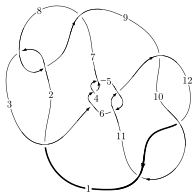
\includegraphics[width=112pt]{../../../GIT/diagram.site/Diagrams/png/1494_12a_0693.png}\\
\ \ \ A knot diagram\footnotemark}&
\allowdisplaybreaks
\textbf{Linearized knot diagam} \\
\cline{2-2}
 &
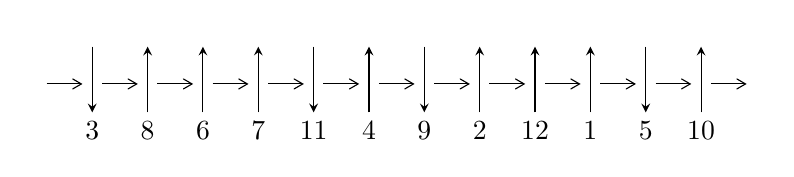
\begin{tikzpicture}[x=20pt, y=17pt]
	% nodes
	\node (C0) at (0, 0) {};
	\node (C1) at (1, 0) {};
	\node (C1U) at (1, +1) {};
	\node (C1D) at (1, -1) {3};

	\node (C2) at (2, 0) {};
	\node (C2U) at (2, +1) {};
	\node (C2D) at (2, -1) {8};

	\node (C3) at (3, 0) {};
	\node (C3U) at (3, +1) {};
	\node (C3D) at (3, -1) {6};

	\node (C4) at (4, 0) {};
	\node (C4U) at (4, +1) {};
	\node (C4D) at (4, -1) {7};

	\node (C5) at (5, 0) {};
	\node (C5U) at (5, +1) {};
	\node (C5D) at (5, -1) {11};

	\node (C6) at (6, 0) {};
	\node (C6U) at (6, +1) {};
	\node (C6D) at (6, -1) {4};

	\node (C7) at (7, 0) {};
	\node (C7U) at (7, +1) {};
	\node (C7D) at (7, -1) {9};

	\node (C8) at (8, 0) {};
	\node (C8U) at (8, +1) {};
	\node (C8D) at (8, -1) {2};

	\node (C9) at (9, 0) {};
	\node (C9U) at (9, +1) {};
	\node (C9D) at (9, -1) {12};

	\node (C10) at (10, 0) {};
	\node (C10U) at (10, +1) {};
	\node (C10D) at (10, -1) {1};

	\node (C11) at (11, 0) {};
	\node (C11U) at (11, +1) {};
	\node (C11D) at (11, -1) {5};

	\node (C12) at (12, 0) {};
	\node (C12U) at (12, +1) {};
	\node (C12D) at (12, -1) {10};
	\node (C13) at (13, 0) {};

	% arrows
	\draw[->,>={angle 60}]
	(C0) edge (C1) (C1) edge (C2) (C2) edge (C3) (C3) edge (C4) (C4) edge (C5) (C5) edge (C6) (C6) edge (C7) (C7) edge (C8) (C8) edge (C9) (C9) edge (C10) (C10) edge (C11) (C11) edge (C12) (C12) edge (C13) ;	\draw[->,>=stealth]
	(C1U) edge (C1D) (C2D) edge (C2U) (C3D) edge (C3U) (C4D) edge (C4U) (C5U) edge (C5D) (C6D) edge (C6U) (C7U) edge (C7D) (C8D) edge (C8U) (C9D) edge (C9U) (C10D) edge (C10U) (C11U) edge (C11D) (C12D) edge (C12U) ;
	\end{tikzpicture} \\
\hhline{~~} \\& 
\textbf{Solving Sequence} \\ \cline{2-2} 
 &
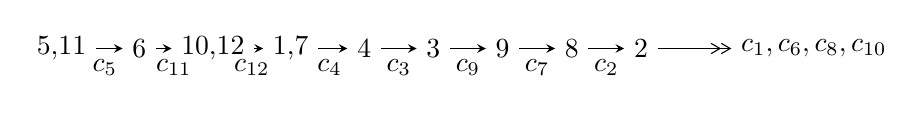
\begin{tikzpicture}[x=25pt, y=7pt]
	% node
	\node (A0) at (-1/8, 0) {5,11};
	\node (A1) at (1, 0) {6};
	\node (A2) at (33/16, 0) {10,12};
	\node (A3) at (51/16, 0) {1,7};
	\node (A4) at (17/4, 0) {4};
	\node (A5) at (21/4, 0) {3};
	\node (A6) at (25/4, 0) {9};
	\node (A7) at (29/4, 0) {8};
	\node (A8) at (33/4, 0) {2};
	\node (C1) at (1/2, -1) {$c_{5}$};
	\node (C2) at (3/2, -1) {$c_{11}$};
	\node (C3) at (21/8, -1) {$c_{12}$};
	\node (C4) at (15/4, -1) {$c_{4}$};
	\node (C5) at (19/4, -1) {$c_{3}$};
	\node (C6) at (23/4, -1) {$c_{9}$};
	\node (C7) at (27/4, -1) {$c_{7}$};
	\node (C8) at (31/4, -1) {$c_{2}$};
	\node (A9) at (43/4, 0) {$c_{1},c_{6},c_{8},c_{10}$};

	% edge
	\draw[->,>=stealth]	
	(A0) edge (A1) (A1) edge (A2) (A2) edge (A3) (A3) edge (A4) (A4) edge (A5) (A5) edge (A6) (A6) edge (A7) (A7) edge (A8) ;
	\draw[->>,>={angle 60}]	
	(A8) edge (A9);
\end{tikzpicture} \\ 

\end{tabular} \\

\footnotetext{
The image of knot diagram is generated by the software ``\textbf{Draw programme}" developed by Andrew Bartholomew(\url{http://www.layer8.co.uk/maths/draw/index.htm\#Running-draw}), where we modified some parts for our purpose(\url{https://github.com/CATsTAILs/LinksPainter}).
}\phantom \\ \newline 
\centering \textbf{Ideals for irreducible components\footnotemark of $X_{\text{par}}$} 
 
\begin{align*}
I^u_{1}&=\langle 
3.03402\times10^{43} u^{32}-2.41482\times10^{44} u^{31}+\cdots+8.30969\times10^{46} d-2.35468\times10^{45},\\
\phantom{I^u_{1}}&\phantom{= \langle  }-1.63168\times10^{45} u^{32}+5.79263\times10^{45} u^{31}+\cdots+1.66194\times10^{47} c+8.26721\times10^{46},\\
\phantom{I^u_{1}}&\phantom{= \langle  }2.98338\times10^{44} u^{32}-6.07211\times10^{44} u^{31}+\cdots+8.30969\times10^{46} b+2.51360\times10^{46},\\
\phantom{I^u_{1}}&\phantom{= \langle  }1.47168\times10^{44} u^{32}-3.80823\times10^{44} u^{31}+\cdots+1.66194\times10^{47} a-1.40982\times10^{47},\;u^{33}-3 u^{32}+\cdots-32 u+32\rangle \\
I^u_{2}&=\langle 
-43643176926349 u^{24}-6533209487727 u^{23}+\cdots+36953350808552 d-173010685681858,\\
\phantom{I^u_{2}}&\phantom{= \langle  }-25166501522073 u^{24} a+34404839224211 u^{24}+\cdots-99103984064754 a+136057334873306,\\
\phantom{I^u_{2}}&\phantom{= \langle  }-18554983719311 u^{24} a+8394493620023 u^{24}+\cdots+50333003044146 a-30523951539978,\\
\phantom{I^u_{2}}&\phantom{= \langle  }-86505342840929 u^{24} a+33387065157365 u^{24}+\cdots+716188465355062 a-526188833960766,\\
\phantom{I^u_{2}}&\phantom{= \langle  }u^{25}+u^{24}+\cdots+4 u-4\rangle \\
\\
I^v_{1}&=\langle 
a,\;d,\;c- v,\;b+1,\;v^2- v+1\rangle \\
I^v_{2}&=\langle 
c,\;d+v-1,\;b,\;a-1,\;v^2- v+1\rangle \\
I^v_{3}&=\langle 
a,\;d+1,\;c- a+1,\;b+1,\;v+1\rangle \\
I^v_{4}&=\langle 
a,\;a^2 d+c^2 v-2 v^2 c+v^3+2 c a+c v-2 a v- v^2+a+v,\;d v-1,\\
\phantom{I^v_{4}}&\phantom{= \langle  }c^2 v^2-2 v^3 c+v^4+2 c a v+v^2 c-2 v^2 a- v^3+a^2+a v+v^2,\;b+1\rangle \\
\end{align*}
\raggedright * 5 irreducible components of $\dim_{\mathbb{C}}=0$, with total 88 representations.\\
\raggedright * 1 irreducible components of $\dim_{\mathbb{C}}=1$ \\
\footnotetext{All coefficients of polynomials are rational numbers. But the coefficients are sometimes approximated in decimal forms when there is not enough margin.}
\newpage
\renewcommand{\arraystretch}{1}
\centering \section*{I. $I^u_{1}= \langle 3.03\times10^{43} u^{32}-2.41\times10^{44} u^{31}+\cdots+8.31\times10^{46} d-2.35\times10^{45},\;-1.63\times10^{45} u^{32}+5.79\times10^{45} u^{31}+\cdots+1.66\times10^{47} c+8.27\times10^{46},\;2.98\times10^{44} u^{32}-6.07\times10^{44} u^{31}+\cdots+8.31\times10^{46} b+2.51\times10^{46},\;1.47\times10^{44} u^{32}-3.81\times10^{44} u^{31}+\cdots+1.66\times10^{47} a-1.41\times10^{47},\;u^{33}-3 u^{32}+\cdots-32 u+32 \rangle$}
\flushleft \textbf{(i) Arc colorings}\\
\begin{tabular}{m{7pt} m{180pt} m{7pt} m{180pt} }
\flushright $a_{5}=$&$\begin{pmatrix}1\\0\end{pmatrix}$ \\
\flushright $a_{11}=$&$\begin{pmatrix}0\\u\end{pmatrix}$ \\
\flushright $a_{6}=$&$\begin{pmatrix}1\\u^2\end{pmatrix}$ \\
\flushright $a_{10}=$&$\begin{pmatrix}0.00981792 u^{32}-0.0348547 u^{31}+\cdots+1.28086 u-0.497444\\-0.000365118 u^{32}+0.00290603 u^{31}+\cdots+0.819964 u+0.0283366\end{pmatrix}$ \\
\flushright $a_{12}=$&$\begin{pmatrix}- u\\u\end{pmatrix}$ \\
\flushright $a_{1}=$&$\begin{pmatrix}-0.00945281 u^{32}+0.0319487 u^{31}+\cdots-2.10082 u+0.469107\\-0.000365118 u^{32}+0.00290603 u^{31}+\cdots+0.819964 u+0.0283366\end{pmatrix}$ \\
\flushright $a_{7}=$&$\begin{pmatrix}-0.000885519 u^{32}+0.00229144 u^{31}+\cdots-0.0914785 u+0.848301\\-0.00359025 u^{32}+0.00730726 u^{31}+\cdots-0.166618 u-0.302490\end{pmatrix}$ \\
\flushright $a_{4}=$&$\begin{pmatrix}-0.000885519 u^{32}+0.00229144 u^{31}+\cdots-0.0914785 u+0.848301\\0.00540092 u^{32}-0.0113739 u^{31}+\cdots+0.183270 u+0.314174\end{pmatrix}$ \\
\flushright $a_{3}=$&$\begin{pmatrix}-0.00447577 u^{32}+0.00959870 u^{31}+\cdots-0.258096 u+0.545811\\0.00661052 u^{32}-0.0132031 u^{31}+\cdots+0.187327 u+0.425005\end{pmatrix}$ \\
\flushright $a_{9}=$&$\begin{pmatrix}0.0132814 u^{32}-0.0464547 u^{31}+\cdots+1.69824 u-0.612332\\-0.00382860 u^{32}+0.0145061 u^{31}+\cdots+0.402587 u+0.143225\end{pmatrix}$ \\
\flushright $a_{8}=$&$\begin{pmatrix}-0.0199599 u^{32}+0.0470707 u^{31}+\cdots-1.09062 u+0.264873\\0.00406824 u^{32}-0.00955037 u^{31}+\cdots-0.124182 u-0.479897\end{pmatrix}$ \\
\flushright $a_{2}=$&$\begin{pmatrix}-0.0149968 u^{32}+0.0409221 u^{31}+\cdots-2.43207 u+0.604078\\-0.0128090 u^{32}+0.0440976 u^{31}+\cdots-0.373843 u+0.638717\end{pmatrix}$\\&\end{tabular}
\flushleft \textbf{(ii) Obstruction class $= -1$}\\~\\
\flushleft \textbf{(iii) Cusp Shapes $= 0.0605080 u^{32}-0.0513753 u^{31}+\cdots-7.44134 u+11.1534$}\\~\\
\newpage\renewcommand{\arraystretch}{1}
\flushleft \textbf{(iv) u-Polynomials at the component}\newline \\
\begin{tabular}{m{50pt}|m{274pt}}
Crossings & \hspace{64pt}u-Polynomials at each crossing \\
\hline $$\begin{aligned}c_{1},c_{7}\end{aligned}$$&$\begin{aligned}
&u^{33}+11 u^{32}+\cdots+8 u-16
\end{aligned}$\\
\hline $$\begin{aligned}c_{2},c_{8}\end{aligned}$$&$\begin{aligned}
&u^{33}+u^{32}+\cdots-12 u+4
\end{aligned}$\\
\hline $$\begin{aligned}c_{3},c_{4},c_{6}\\c_{9},c_{10},c_{12}\end{aligned}$$&$\begin{aligned}
&u^{33}+5 u^{32}+\cdots-7 u^2-1
\end{aligned}$\\
\hline $$\begin{aligned}c_{5},c_{11}\end{aligned}$$&$\begin{aligned}
&u^{33}-3 u^{32}+\cdots-32 u+32
\end{aligned}$\\
\hline
\end{tabular}\\~\\
\newpage\renewcommand{\arraystretch}{1}
\flushleft \textbf{(v) Riley Polynomials at the component}\newline \\
\begin{tabular}{m{50pt}|m{274pt}}
Crossings & \hspace{64pt}Riley Polynomials at each crossing \\
\hline $$\begin{aligned}c_{1},c_{7}\end{aligned}$$&$\begin{aligned}
&y^{33}+23 y^{32}+\cdots-14304 y-256
\end{aligned}$\\
\hline $$\begin{aligned}c_{2},c_{8}\end{aligned}$$&$\begin{aligned}
&y^{33}+11 y^{32}+\cdots+8 y-16
\end{aligned}$\\
\hline $$\begin{aligned}c_{3},c_{4},c_{6}\\c_{9},c_{10},c_{12}\end{aligned}$$&$\begin{aligned}
&y^{33}-39 y^{32}+\cdots-14 y-1
\end{aligned}$\\
\hline $$\begin{aligned}c_{5},c_{11}\end{aligned}$$&$\begin{aligned}
&y^{33}+15 y^{32}+\cdots-6144 y-1024
\end{aligned}$\\
\hline
\end{tabular}\\~\\
\newpage\flushleft \textbf{(vi) Complex Volumes and Cusp Shapes}
$$\begin{array}{c|c|c}  
\text{Solutions to }I^u_{1}& \I (\text{vol} + \sqrt{-1}CS) & \text{Cusp shape}\\
 \hline 
\begin{aligned}
u &= \phantom{-}0.979372 + 0.273800 I \\
a &= \phantom{-}0.431028 - 0.024061 I \\
b &= -1.312830 - 0.129109 I \\
c &= -1.70621 + 0.13086 I \\
d &= \phantom{-}0.428725 + 0.094450 I\end{aligned}
 & \phantom{-}4.01193 + 3.40996 I & \phantom{-}6.93635 - 3.61829 I \\ \hline\begin{aligned}
u &= \phantom{-}0.979372 - 0.273800 I \\
a &= \phantom{-}0.431028 + 0.024061 I \\
b &= -1.312830 + 0.129109 I \\
c &= -1.70621 - 0.13086 I \\
d &= \phantom{-}0.428725 - 0.094450 I\end{aligned}
 & \phantom{-}4.01193 - 3.40996 I & \phantom{-}6.93635 + 3.61829 I \\ \hline\begin{aligned}
u &= \phantom{-}0.581985 + 0.777781 I \\
a &= \phantom{-}0.666890 + 0.389948 I \\
b &= -0.117441 + 0.653397 I \\
c &= \phantom{-}0.381291 - 0.245865 I \\
d &= \phantom{-}0.084826 + 0.745638 I\end{aligned}
 & -3.19812 - 2.28214 I & -2.55468 + 4.65224 I \\ \hline\begin{aligned}
u &= \phantom{-}0.581985 - 0.777781 I \\
a &= \phantom{-}0.666890 - 0.389948 I \\
b &= -0.117441 - 0.653397 I \\
c &= \phantom{-}0.381291 + 0.245865 I \\
d &= \phantom{-}0.084826 - 0.745638 I\end{aligned}
 & -3.19812 + 2.28214 I & -2.55468 - 4.65224 I \\ \hline\begin{aligned}
u &= -0.342726 + 1.062970 I \\
a &= \phantom{-}0.557825 - 0.285941 I \\
b &= -0.419652 - 0.727712 I \\
c &= -0.617597 - 0.133391 I \\
d &= \phantom{-}0.112766 + 0.690951 I\end{aligned}
 & \phantom{-}2.46500 + 1.75021 I & \phantom{-}7.36804 - 3.35767 I \\ \hline\begin{aligned}
u &= -0.342726 - 1.062970 I \\
a &= \phantom{-}0.557825 + 0.285941 I \\
b &= -0.419652 + 0.727712 I \\
c &= -0.617597 + 0.133391 I \\
d &= \phantom{-}0.112766 - 0.690951 I\end{aligned}
 & \phantom{-}2.46500 - 1.75021 I & \phantom{-}7.36804 + 3.35767 I\\
 \hline 
 \end{array}$$\newpage$$\begin{array}{c|c|c}  
\text{Solutions to }I^u_{1}& \I (\text{vol} + \sqrt{-1}CS) & \text{Cusp shape}\\
 \hline 
\begin{aligned}
u &= -1.16826\phantom{ +0.000000I} \\
a &= \phantom{-}0.415930\phantom{ +0.000000I} \\
b &= -1.40425\phantom{ +0.000000I} \\
c &= \phantom{-}1.68792\phantom{ +0.000000I} \\
d &= -0.485914\phantom{ +0.000000I}\end{aligned}
 & \phantom{-}7.47395\phantom{ +0.000000I} & \phantom{-}12.4850\phantom{ +0.000000I} \\ \hline\begin{aligned}
u &= \phantom{-}0.464136 + 1.103860 I \\
a &= \phantom{-}0.545028 + 0.324179 I \\
b &= -0.355294 + 0.806119 I \\
c &= \phantom{-}0.610442 - 0.217661 I \\
d &= -0.104881 + 0.752097 I\end{aligned}
 & \phantom{-}1.74788 - 7.33440 I & \phantom{-}5.47919 + 8.14278 I \\ \hline\begin{aligned}
u &= \phantom{-}0.464136 - 1.103860 I \\
a &= \phantom{-}0.545028 - 0.324179 I \\
b &= -0.355294 - 0.806119 I \\
c &= \phantom{-}0.610442 + 0.217661 I \\
d &= -0.104881 - 0.752097 I\end{aligned}
 & \phantom{-}1.74788 + 7.33440 I & \phantom{-}5.47919 - 8.14278 I \\ \hline\begin{aligned}
u &= \phantom{-}0.635877 + 0.397843 I \\
a &= \phantom{-}0.923878 + 0.490787 I \\
b &= \phantom{-}0.155830 + 0.448444 I \\
c &= \phantom{-}0.101013 - 0.282995 I \\
d &= \phantom{-}0.392216 + 0.679638 I\end{aligned}
 & -0.42221 + 2.98824 I & -0.68495 - 3.66701 I \\ \hline\begin{aligned}
u &= \phantom{-}0.635877 - 0.397843 I \\
a &= \phantom{-}0.923878 - 0.490787 I \\
b &= \phantom{-}0.155830 - 0.448444 I \\
c &= \phantom{-}0.101013 + 0.282995 I \\
d &= \phantom{-}0.392216 - 0.679638 I\end{aligned}
 & -0.42221 - 2.98824 I & -0.68495 + 3.66701 I \\ \hline\begin{aligned}
u &= -0.239228 + 0.607577 I \\
a &= \phantom{-}0.750526 - 0.191152 I \\
b &= -0.251234 - 0.318679 I \\
c &= -0.249740 + 0.035069 I \\
d &= -0.063407 + 0.501731 I\end{aligned}
 & \phantom{-}0.292144 + 0.942663 I & \phantom{-}5.66111 - 7.03214 I\\
 \hline 
 \end{array}$$\newpage$$\begin{array}{c|c|c}  
\text{Solutions to }I^u_{1}& \I (\text{vol} + \sqrt{-1}CS) & \text{Cusp shape}\\
 \hline 
\begin{aligned}
u &= -0.239228 - 0.607577 I \\
a &= \phantom{-}0.750526 + 0.191152 I \\
b &= -0.251234 + 0.318679 I \\
c &= -0.249740 - 0.035069 I \\
d &= -0.063407 - 0.501731 I\end{aligned}
 & \phantom{-}0.292144 - 0.942663 I & \phantom{-}5.66111 + 7.03214 I \\ \hline\begin{aligned}
u &= \phantom{-}0.351447 + 1.312440 I \\
a &= -1.87607 - 0.66709 I \\
b &= \phantom{-}1.47320 - 0.16826 I \\
c &= -0.05533 + 1.61726 I \\
d &= \phantom{-}0.21618 - 2.69668 I\end{aligned}
 & \phantom{-}9.06107 - 0.86504 I & \phantom{-}11.01805 + 0.17133 I \\ \hline\begin{aligned}
u &= \phantom{-}0.351447 - 1.312440 I \\
a &= -1.87607 + 0.66709 I \\
b &= \phantom{-}1.47320 + 0.16826 I \\
c &= -0.05533 - 1.61726 I \\
d &= \phantom{-}0.21618 + 2.69668 I\end{aligned}
 & \phantom{-}9.06107 + 0.86504 I & \phantom{-}11.01805 - 0.17133 I \\ \hline\begin{aligned}
u &= \phantom{-}0.611782 + 1.268620 I \\
a &= -1.54743 - 1.00939 I \\
b &= \phantom{-}1.45334 - 0.29571 I \\
c &= -0.07474 + 1.55998 I \\
d &= \phantom{-}0.33385 - 2.58063 I\end{aligned}
 & \phantom{-}7.09875 - 9.27148 I & \phantom{-}8.26421 + 6.23171 I \\ \hline\begin{aligned}
u &= \phantom{-}0.611782 - 1.268620 I \\
a &= -1.54743 + 1.00939 I \\
b &= \phantom{-}1.45334 + 0.29571 I \\
c &= -0.07474 - 1.55998 I \\
d &= \phantom{-}0.33385 + 2.58063 I\end{aligned}
 & \phantom{-}7.09875 + 9.27148 I & \phantom{-}8.26421 - 6.23171 I \\ \hline\begin{aligned}
u &= \phantom{-}0.053785 + 0.584876 I \\
a &= \phantom{-}0.567133 - 0.028165 I \\
b &= -0.758918 - 0.087353 I \\
c &= -0.313400 + 0.942882 I \\
d &= \phantom{-}0.046976 + 0.330187 I\end{aligned}
 & \phantom{-}2.76296 + 2.31801 I & \phantom{-}12.30250 - 4.19824 I\\
 \hline 
 \end{array}$$\newpage$$\begin{array}{c|c|c}  
\text{Solutions to }I^u_{1}& \I (\text{vol} + \sqrt{-1}CS) & \text{Cusp shape}\\
 \hline 
\begin{aligned}
u &= \phantom{-}0.053785 - 0.584876 I \\
a &= \phantom{-}0.567133 + 0.028165 I \\
b &= -0.758918 + 0.087353 I \\
c &= -0.313400 - 0.942882 I \\
d &= \phantom{-}0.046976 - 0.330187 I\end{aligned}
 & \phantom{-}2.76296 - 2.31801 I & \phantom{-}12.30250 + 4.19824 I \\ \hline\begin{aligned}
u &= -1.38673 + 0.43185 I \\
a &= \phantom{-}0.395798 + 0.032608 I \\
b &= -1.50951 + 0.20675 I \\
c &= \phantom{-}1.59758 + 0.04740 I \\
d &= -0.562946 + 0.125707 I\end{aligned}
 & \phantom{-}11.58920 - 2.62797 I & \phantom{-}12.22236 + 0.42879 I \\ \hline\begin{aligned}
u &= -1.38673 - 0.43185 I \\
a &= \phantom{-}0.395798 - 0.032608 I \\
b &= -1.50951 - 0.20675 I \\
c &= \phantom{-}1.59758 - 0.04740 I \\
d &= -0.562946 - 0.125707 I\end{aligned}
 & \phantom{-}11.58920 + 2.62797 I & \phantom{-}12.22236 - 0.42879 I \\ \hline\begin{aligned}
u &= -0.489796 + 0.230188 I \\
a &= \phantom{-}1.111610 - 0.308664 I \\
b &= \phantom{-}0.164799 - 0.231913 I \\
c &= \phantom{-}0.015550 - 0.148753 I \\
d &= -0.473411 + 0.407061 I\end{aligned}
 & \phantom{-}0.15528 + 1.56621 I & -1.22779 - 2.98994 I \\ \hline\begin{aligned}
u &= -0.489796 - 0.230188 I \\
a &= \phantom{-}1.111610 + 0.308664 I \\
b &= \phantom{-}0.164799 + 0.231913 I \\
c &= \phantom{-}0.015550 + 0.148753 I \\
d &= -0.473411 - 0.407061 I\end{aligned}
 & \phantom{-}0.15528 - 1.56621 I & -1.22779 + 2.98994 I \\ \hline\begin{aligned}
u &= \phantom{-}1.35730 + 0.53891 I \\
a &= \phantom{-}0.396350 - 0.041125 I \\
b &= -1.49615 - 0.25900 I \\
c &= -1.57777 + 0.05545 I \\
d &= \phantom{-}0.560127 + 0.157777 I\end{aligned}
 & \phantom{-}10.79550 + 8.72073 I & \phantom{-}10.94592 - 5.35160 I\\
 \hline 
 \end{array}$$\newpage$$\begin{array}{c|c|c}  
\text{Solutions to }I^u_{1}& \I (\text{vol} + \sqrt{-1}CS) & \text{Cusp shape}\\
 \hline 
\begin{aligned}
u &= \phantom{-}1.35730 - 0.53891 I \\
a &= \phantom{-}0.396350 + 0.041125 I \\
b &= -1.49615 + 0.25900 I \\
c &= -1.57777 - 0.05545 I \\
d &= \phantom{-}0.560127 - 0.157777 I\end{aligned}
 & \phantom{-}10.79550 - 8.72073 I & \phantom{-}10.94592 + 5.35160 I \\ \hline\begin{aligned}
u &= -0.48684 + 1.39736 I \\
a &= -1.61091 + 0.72954 I \\
b &= \phantom{-}1.51512 + 0.23328 I \\
c &= \phantom{-}0.04717 + 1.58742 I \\
d &= -0.23517 - 2.60619 I\end{aligned}
 & \phantom{-}12.10590 + 5.85939 I & \phantom{-}13.7252 - 3.8290 I \\ \hline\begin{aligned}
u &= -0.48684 - 1.39736 I \\
a &= -1.61091 - 0.72954 I \\
b &= \phantom{-}1.51512 - 0.23328 I \\
c &= \phantom{-}0.04717 - 1.58742 I \\
d &= -0.23517 + 2.60619 I\end{aligned}
 & \phantom{-}12.10590 - 5.85939 I & \phantom{-}13.7252 + 3.8290 I \\ \hline\begin{aligned}
u &= \phantom{-}0.82581 + 1.33817 I \\
a &= -1.22197 - 0.99602 I \\
b &= \phantom{-}1.49169 - 0.40077 I \\
c &= -0.04243 + 1.51660 I \\
d &= \phantom{-}0.32373 - 2.45773 I\end{aligned}
 & \phantom{-}13.4411 - 16.4286 I & \phantom{-}10.77382 + 8.75984 I \\ \hline\begin{aligned}
u &= \phantom{-}0.82581 - 1.33817 I \\
a &= -1.22197 + 0.99602 I \\
b &= \phantom{-}1.49169 + 0.40077 I \\
c &= -0.04243 - 1.51660 I \\
d &= \phantom{-}0.32373 + 2.45773 I\end{aligned}
 & \phantom{-}13.4411 + 16.4286 I & \phantom{-}10.77382 - 8.75984 I \\ \hline\begin{aligned}
u &= -0.77347 + 1.38729 I \\
a &= -1.27234 + 0.92357 I \\
b &= \phantom{-}1.51473 + 0.37364 I \\
c &= \phantom{-}0.03820 + 1.53196 I \\
d &= -0.29714 - 2.47946 I\end{aligned}
 & \phantom{-}14.7439 + 10.2508 I & \phantom{-}12.57547 - 4.19472 I\\
 \hline 
 \end{array}$$\newpage$$\begin{array}{c|c|c}  
\text{Solutions to }I^u_{1}& \I (\text{vol} + \sqrt{-1}CS) & \text{Cusp shape}\\
 \hline 
\begin{aligned}
u &= -0.77347 - 1.38729 I \\
a &= -1.27234 - 0.92357 I \\
b &= \phantom{-}1.51473 - 0.37364 I \\
c &= \phantom{-}0.03820 - 1.53196 I \\
d &= -0.29714 + 2.47946 I\end{aligned}
 & \phantom{-}14.7439 - 10.2508 I & \phantom{-}12.57547 + 4.19472 I \\ \hline\begin{aligned}
u &= -0.05858 + 1.69521 I \\
a &= -1.52532 + 0.06419 I \\
b &= \phantom{-}1.65444 + 0.02754 I \\
c &= \phantom{-}0.00202 + 1.61414 I \\
d &= -0.01947 - 2.58949 I\end{aligned}
 & -19.6551 + 3.2714 I & \phantom{-}13.9526 - 2.4448 I \\ \hline\begin{aligned}
u &= -0.05858 - 1.69521 I \\
a &= -1.52532 - 0.06419 I \\
b &= \phantom{-}1.65444 - 0.02754 I \\
c &= \phantom{-}0.00202 - 1.61414 I \\
d &= -0.01947 + 2.58949 I\end{aligned}
 & -19.6551 - 3.2714 I & \phantom{-}13.9526 + 2.4448 I\\
 \hline 
 \end{array}$$\newpage\newpage\renewcommand{\arraystretch}{1}
\centering \section*{II. $I^u_{2}= \langle -4.36\times10^{13} u^{24}-6.53\times10^{12} u^{23}+\cdots+3.70\times10^{13} d-1.73\times10^{14},\;-2.52\times10^{13} a u^{24}+3.44\times10^{13} u^{24}+\cdots-9.91\times10^{13} a+1.36\times10^{14},\;-1.86\times10^{13} a u^{24}+8.39\times10^{12} u^{24}+\cdots+5.03\times10^{13} a-3.05\times10^{13},\;-8.65\times10^{13} a u^{24}+3.34\times10^{13} u^{24}+\cdots+7.16\times10^{14} a-5.26\times10^{14},\;u^{25}+u^{24}+\cdots+4 u-4 \rangle$}
\flushleft \textbf{(i) Arc colorings}\\
\begin{tabular}{m{7pt} m{180pt} m{7pt} m{180pt} }
\flushright $a_{5}=$&$\begin{pmatrix}1\\0\end{pmatrix}$ \\
\flushright $a_{11}=$&$\begin{pmatrix}0\\u\end{pmatrix}$ \\
\flushright $a_{6}=$&$\begin{pmatrix}1\\u^2\end{pmatrix}$ \\
\flushright $a_{10}=$&$\begin{pmatrix}0.681034 a u^{24}-0.931034 u^{24}+\cdots+2.68187 a-3.68187\\1.18103 u^{24}+0.176796 u^{23}+\cdots-14.3723 u+4.68187\end{pmatrix}$ \\
\flushright $a_{12}=$&$\begin{pmatrix}- u\\u\end{pmatrix}$ \\
\flushright $a_{1}=$&$\begin{pmatrix}-0.681034 a u^{24}-0.250000 u^{24}+\cdots-2.68187 a-1\\1.18103 u^{24}+0.176796 u^{23}+\cdots-14.3723 u+4.68187\end{pmatrix}$ \\
\flushright $a_{7}=$&$\begin{pmatrix}a\\1.00424 a u^{24}-0.454329 u^{24}+\cdots-2.72414 a+1.65203\end{pmatrix}$ \\
\flushright $a_{4}=$&$\begin{pmatrix}a\\-1.00424 a u^{24}+0.454329 u^{24}+\cdots+2.72414 a-1.65203\end{pmatrix}$ \\
\flushright $a_{3}=$&$\begin{pmatrix}1.00424 a u^{24}-0.454329 u^{24}+\cdots-1.72414 a+1.65203\\-1.99712 a u^{24}+0.930056 u^{24}+\cdots+4.50730 a-3.40772\end{pmatrix}$ \\
\flushright $a_{9}=$&$\begin{pmatrix}1.12683 a u^{24}-0.931034 u^{24}+\cdots+6.69882 a-3.68187\\-0.445792 a u^{24}+1.18103 u^{24}+\cdots-4.01695 a+4.68187\end{pmatrix}$ \\
\flushright $a_{8}=$&$\begin{pmatrix}-2.44203 a u^{24}+1.16427 u^{24}+\cdots+6.39909 a+0.185751\\2.42063 a u^{24}-1.33567 u^{24}+\cdots-6.29543 a-3.15467\end{pmatrix}$ \\
\flushright $a_{2}=$&$\begin{pmatrix}-1.57386 a u^{24}+0.195792 u^{24}+\cdots-7.91615 a+3.01695\\0.638749 a u^{24}+0.561007 u^{24}+\cdots+9.76810 a-3.30659\end{pmatrix}$\\&\end{tabular}
\flushleft \textbf{(ii) Obstruction class $= -1$}\\~\\
\flushleft \textbf{(iii) Cusp Shapes $= -\frac{6062761600965}{9238337702138} u^{24}+\frac{3225176474347}{9238337702138} u^{23}+\cdots+\frac{61042729884201}{9238337702138} u+\frac{27155343409896}{4619168851069}$}\\~\\
\newpage\renewcommand{\arraystretch}{1}
\flushleft \textbf{(iv) u-Polynomials at the component}\newline \\
\begin{tabular}{m{50pt}|m{274pt}}
Crossings & \hspace{64pt}u-Polynomials at each crossing \\
\hline $$\begin{aligned}c_{1},c_{7}\end{aligned}$$&$\begin{aligned}
&(u^{25}+8 u^{24}+\cdots+11 u-1)^{2}
\end{aligned}$\\
\hline $$\begin{aligned}c_{2}\end{aligned}$$&$\begin{aligned}
&(u^{25}+2 u^{24}+\cdots+3 u+1)^{2}
\end{aligned}$\\
\hline $$\begin{aligned}c_{3},c_{4},c_{9}\end{aligned}$$&$\begin{aligned}
&u^{50}+3 u^{49}+\cdots+24 u-16
\end{aligned}$\\
\hline $$\begin{aligned}c_{5}\end{aligned}$$&$\begin{aligned}
&(u^{25}+u^{24}+\cdots+4 u-4)^{2}
\end{aligned}$\\
\hline $$\begin{aligned}c_{6},c_{10},c_{12}\end{aligned}$$&$\begin{aligned}
&- u^{50}+3 u^{49}+\cdots+24 u+16
\end{aligned}$\\
\hline $$\begin{aligned}c_{8}\end{aligned}$$&$\begin{aligned}
&(u^{25}-2 u^{24}+\cdots+3 u-1)^{2}
\end{aligned}$\\
\hline $$\begin{aligned}c_{11}\end{aligned}$$&$\begin{aligned}
&(u^{25}- u^{24}+\cdots+4 u+4)^{2}
\end{aligned}$\\
\hline
\end{tabular}\\~\\
\newpage\renewcommand{\arraystretch}{1}
\flushleft \textbf{(v) Riley Polynomials at the component}\newline \\
\begin{tabular}{m{50pt}|m{274pt}}
Crossings & \hspace{64pt}Riley Polynomials at each crossing \\
\hline $$\begin{aligned}c_{1},c_{7}\end{aligned}$$&$\begin{aligned}
&(y^{25}+20 y^{24}+\cdots+251 y-1)^{2}
\end{aligned}$\\
\hline $$\begin{aligned}c_{2},c_{8}\end{aligned}$$&$\begin{aligned}
&(y^{25}+8 y^{24}+\cdots+11 y-1)^{2}
\end{aligned}$\\
\hline $$\begin{aligned}c_{3},c_{4},c_{6}\\c_{9},c_{10},c_{12}\end{aligned}$$&$\begin{aligned}
&y^{50}-39 y^{49}+\cdots-3872 y+256
\end{aligned}$\\
\hline $$\begin{aligned}c_{5},c_{11}\end{aligned}$$&$\begin{aligned}
&(y^{25}+15 y^{24}+\cdots-88 y-16)^{2}
\end{aligned}$\\
\hline
\end{tabular}\\~\\
\newpage\flushleft \textbf{(vi) Complex Volumes and Cusp Shapes}
$$\begin{array}{c|c|c}  
\text{Solutions to }I^u_{2}& \I (\text{vol} + \sqrt{-1}CS) & \text{Cusp shape}\\
 \hline 
\begin{aligned}
u &= -0.111975 + 0.962557 I \\
a &= \phantom{-}0.567856 - 0.205094 I \\
b &= -0.557801 - 0.562636 I \\
c &= \phantom{-}0.819383 + 0.216893 I \\
d &= -0.206986 + 0.489964 I\end{aligned}
 & \phantom{-}3.08820 + 2.66172 I & \phantom{-}9.28523 - 3.57661 I \\ \hline\begin{aligned}
u &= -0.111975 + 0.962557 I \\
a &= \phantom{-}0.526908 + 0.153743 I \\
b &= -0.748963 + 0.510317 I \\
c &= -0.644034 + 0.069293 I \\
d &= \phantom{-}0.133829 + 0.569559 I\end{aligned}
 & \phantom{-}3.08820 + 2.66172 I & \phantom{-}9.28523 - 3.57661 I \\ \hline\begin{aligned}
u &= -0.111975 - 0.962557 I \\
a &= \phantom{-}0.567856 + 0.205094 I \\
b &= -0.557801 + 0.562636 I \\
c &= \phantom{-}0.819383 - 0.216893 I \\
d &= -0.206986 - 0.489964 I\end{aligned}
 & \phantom{-}3.08820 - 2.66172 I & \phantom{-}9.28523 + 3.57661 I \\ \hline\begin{aligned}
u &= -0.111975 - 0.962557 I \\
a &= \phantom{-}0.526908 - 0.153743 I \\
b &= -0.748963 - 0.510317 I \\
c &= -0.644034 - 0.069293 I \\
d &= \phantom{-}0.133829 - 0.569559 I\end{aligned}
 & \phantom{-}3.08820 - 2.66172 I & \phantom{-}9.28523 + 3.57661 I \\ \hline\begin{aligned}
u &= \phantom{-}1.061780 + 0.135314 I \\
a &= \phantom{-}0.707086 + 1.072640 I \\
b &= \phantom{-}0.571600 + 0.649877 I \\
c &= -1.71425 + 0.05535 I \\
d &= \phantom{-}0.452395 + 0.045198 I\end{aligned}
 & \phantom{-}4.81480 - 0.43356 I & \phantom{-}8.91196 - 0.04506 I \\ \hline\begin{aligned}
u &= \phantom{-}1.061780 + 0.135314 I \\
a &= \phantom{-}0.424600 - 0.011543 I \\
b &= -1.353420 - 0.063981 I \\
c &= \phantom{-}0.000864 - 0.699820 I \\
d &= \phantom{-}0.605628 + 1.234590 I\end{aligned}
 & \phantom{-}4.81480 - 0.43356 I & \phantom{-}8.91196 - 0.04506 I\\
 \hline 
 \end{array}$$\newpage$$\begin{array}{c|c|c}  
\text{Solutions to }I^u_{2}& \I (\text{vol} + \sqrt{-1}CS) & \text{Cusp shape}\\
 \hline 
\begin{aligned}
u &= \phantom{-}1.061780 - 0.135314 I \\
a &= \phantom{-}0.707086 - 1.072640 I \\
b &= \phantom{-}0.571600 - 0.649877 I \\
c &= -1.71425 - 0.05535 I \\
d &= \phantom{-}0.452395 - 0.045198 I\end{aligned}
 & \phantom{-}4.81480 + 0.43356 I & \phantom{-}8.91196 + 0.04506 I \\ \hline\begin{aligned}
u &= \phantom{-}1.061780 - 0.135314 I \\
a &= \phantom{-}0.424600 + 0.011543 I \\
b &= -1.353420 + 0.063981 I \\
c &= \phantom{-}0.000864 + 0.699820 I \\
d &= \phantom{-}0.605628 - 1.234590 I\end{aligned}
 & \phantom{-}4.81480 + 0.43356 I & \phantom{-}8.91196 + 0.04506 I \\ \hline\begin{aligned}
u &= -0.465035 + 1.033020 I \\
a &= \phantom{-}0.568091 - 0.326292 I \\
b &= -0.323623 - 0.760243 I \\
c &= \phantom{-}0.14931 + 1.61347 I \\
d &= -0.45403 - 2.76996 I\end{aligned}
 & \phantom{-}1.37392 + 5.41987 I & \phantom{-}4.64303 - 6.54919 I \\ \hline\begin{aligned}
u &= -0.465035 + 1.033020 I \\
a &= -2.06507 + 1.36916 I \\
b &= \phantom{-}1.336380 + 0.223022 I \\
c &= -0.567551 - 0.202618 I \\
d &= \phantom{-}0.072882 + 0.738584 I\end{aligned}
 & \phantom{-}1.37392 + 5.41987 I & \phantom{-}4.64303 - 6.54919 I \\ \hline\begin{aligned}
u &= -0.465035 - 1.033020 I \\
a &= \phantom{-}0.568091 + 0.326292 I \\
b &= -0.323623 + 0.760243 I \\
c &= \phantom{-}0.14931 - 1.61347 I \\
d &= -0.45403 + 2.76996 I\end{aligned}
 & \phantom{-}1.37392 - 5.41987 I & \phantom{-}4.64303 + 6.54919 I \\ \hline\begin{aligned}
u &= -0.465035 - 1.033020 I \\
a &= -2.06507 - 1.36916 I \\
b &= \phantom{-}1.336380 - 0.223022 I \\
c &= -0.567551 + 0.202618 I \\
d &= \phantom{-}0.072882 - 0.738584 I\end{aligned}
 & \phantom{-}1.37392 - 5.41987 I & \phantom{-}4.64303 + 6.54919 I\\
 \hline 
 \end{array}$$\newpage$$\begin{array}{c|c|c}  
\text{Solutions to }I^u_{2}& \I (\text{vol} + \sqrt{-1}CS) & \text{Cusp shape}\\
 \hline 
\begin{aligned}
u &= -1.096160 + 0.296196 I \\
a &= \phantom{-}0.650082 - 0.890833 I \\
b &= \phantom{-}0.465476 - 0.732479 I \\
c &= \phantom{-}1.66469 + 0.09733 I \\
d &= -0.468544 + 0.097124 I\end{aligned}
 & \phantom{-}4.43073 - 5.11531 I & \phantom{-}7.81745 + 5.48464 I \\ \hline\begin{aligned}
u &= -1.096160 + 0.296196 I \\
a &= \phantom{-}0.420667 + 0.025066 I \\
b &= -1.368770 + 0.141145 I \\
c &= -0.115286 - 0.653233 I \\
d &= -0.448735 + 1.169050 I\end{aligned}
 & \phantom{-}4.43073 - 5.11531 I & \phantom{-}7.81745 + 5.48464 I \\ \hline\begin{aligned}
u &= -1.096160 - 0.296196 I \\
a &= \phantom{-}0.650082 + 0.890833 I \\
b &= \phantom{-}0.465476 + 0.732479 I \\
c &= \phantom{-}1.66469 - 0.09733 I \\
d &= -0.468544 - 0.097124 I\end{aligned}
 & \phantom{-}4.43073 + 5.11531 I & \phantom{-}7.81745 - 5.48464 I \\ \hline\begin{aligned}
u &= -1.096160 - 0.296196 I \\
a &= \phantom{-}0.420667 - 0.025066 I \\
b &= -1.368770 - 0.141145 I \\
c &= -0.115286 + 0.653233 I \\
d &= -0.448735 - 1.169050 I\end{aligned}
 & \phantom{-}4.43073 + 5.11531 I & \phantom{-}7.81745 - 5.48464 I \\ \hline\begin{aligned}
u &= \phantom{-}0.202658 + 1.122680 I \\
a &= \phantom{-}0.533156 + 0.248104 I \\
b &= -0.541755 + 0.717454 I \\
c &= -0.06617 + 1.68118 I \\
d &= \phantom{-}0.19823 - 2.88839 I\end{aligned}
 & \phantom{-}5.39169 - 2.44039 I & \phantom{-}11.83401 + 3.61173 I \\ \hline\begin{aligned}
u &= \phantom{-}0.202658 + 1.122680 I \\
a &= -2.46070 - 0.62076 I \\
b &= \phantom{-}1.382070 - 0.096385 I \\
c &= \phantom{-}0.705023 - 0.069800 I \\
d &= -0.170493 + 0.648845 I\end{aligned}
 & \phantom{-}5.39169 - 2.44039 I & \phantom{-}11.83401 + 3.61173 I\\
 \hline 
 \end{array}$$\newpage$$\begin{array}{c|c|c}  
\text{Solutions to }I^u_{2}& \I (\text{vol} + \sqrt{-1}CS) & \text{Cusp shape}\\
 \hline 
\begin{aligned}
u &= \phantom{-}0.202658 - 1.122680 I \\
a &= \phantom{-}0.533156 - 0.248104 I \\
b &= -0.541755 - 0.717454 I \\
c &= -0.06617 - 1.68118 I \\
d &= \phantom{-}0.19823 + 2.88839 I\end{aligned}
 & \phantom{-}5.39169 + 2.44039 I & \phantom{-}11.83401 - 3.61173 I \\ \hline\begin{aligned}
u &= \phantom{-}0.202658 - 1.122680 I \\
a &= -2.46070 + 0.62076 I \\
b &= \phantom{-}1.382070 + 0.096385 I \\
c &= \phantom{-}0.705023 + 0.069800 I \\
d &= -0.170493 - 0.648845 I\end{aligned}
 & \phantom{-}5.39169 + 2.44039 I & \phantom{-}11.83401 - 3.61173 I \\ \hline\begin{aligned}
u &= -0.641188 + 0.544744 I \\
a &= \phantom{-}0.797389 - 0.461643 I \\
b &= \phantom{-}0.060728 - 0.543785 I \\
c &= \phantom{-}1.54551 + 0.43011 I \\
d &= -0.325741 + 0.217121 I\end{aligned}
 & -0.175498 - 1.059220 I & \phantom{-}0.606046 + 0.370576 I \\ \hline\begin{aligned}
u &= -0.641188 + 0.544744 I \\
a &= \phantom{-}0.462143 + 0.054007 I \\
b &= -1.134680 + 0.249465 I \\
c &= -0.213681 - 0.284545 I \\
d &= -0.259799 + 0.730373 I\end{aligned}
 & -0.175498 - 1.059220 I & \phantom{-}0.606046 + 0.370576 I \\ \hline\begin{aligned}
u &= -0.641188 - 0.544744 I \\
a &= \phantom{-}0.797389 + 0.461643 I \\
b &= \phantom{-}0.060728 + 0.543785 I \\
c &= \phantom{-}1.54551 - 0.43011 I \\
d &= -0.325741 - 0.217121 I\end{aligned}
 & -0.175498 + 1.059220 I & \phantom{-}0.606046 - 0.370576 I \\ \hline\begin{aligned}
u &= -0.641188 - 0.544744 I \\
a &= \phantom{-}0.462143 - 0.054007 I \\
b &= -1.134680 - 0.249465 I \\
c &= -0.213681 + 0.284545 I \\
d &= -0.259799 - 0.730373 I\end{aligned}
 & -0.175498 + 1.059220 I & \phantom{-}0.606046 - 0.370576 I\\
 \hline 
 \end{array}$$\newpage$$\begin{array}{c|c|c}  
\text{Solutions to }I^u_{2}& \I (\text{vol} + \sqrt{-1}CS) & \text{Cusp shape}\\
 \hline 
\begin{aligned}
u &= -0.082989 + 0.805818 I \\
a &= \phantom{-}0.611223 - 0.162597 I \\
b &= -0.527939 - 0.406461 I \\
c &= \phantom{-}0.07908 + 1.88202 I \\
d &= -0.18925 - 3.40293 I\end{aligned}
 & \phantom{-}2.66645 - 1.39976 I & \phantom{-}8.95722 + 0.06062 I \\ \hline\begin{aligned}
u &= -0.082989 + 0.805818 I \\
a &= -4.15470 + 0.66274 I \\
b &= \phantom{-}1.234720 + 0.037441 I \\
c &= -0.512649 + 0.193657 I \\
d &= \phantom{-}0.080299 + 0.506028 I\end{aligned}
 & \phantom{-}2.66645 - 1.39976 I & \phantom{-}8.95722 + 0.06062 I \\ \hline\begin{aligned}
u &= -0.082989 - 0.805818 I \\
a &= \phantom{-}0.611223 + 0.162597 I \\
b &= -0.527939 + 0.406461 I \\
c &= \phantom{-}0.07908 - 1.88202 I \\
d &= -0.18925 + 3.40293 I\end{aligned}
 & \phantom{-}2.66645 + 1.39976 I & \phantom{-}8.95722 - 0.06062 I \\ \hline\begin{aligned}
u &= -0.082989 - 0.805818 I \\
a &= -4.15470 - 0.66274 I \\
b &= \phantom{-}1.234720 - 0.037441 I \\
c &= -0.512649 - 0.193657 I \\
d &= \phantom{-}0.080299 - 0.506028 I\end{aligned}
 & \phantom{-}2.66645 + 1.39976 I & \phantom{-}8.95722 - 0.06062 I \\ \hline\begin{aligned}
u &= \phantom{-}0.340493 + 0.559321 I \\
a &= \phantom{-}0.502139 - 0.055131 I \\
b &= -0.967761 - 0.216045 I \\
c &= -0.55582 + 1.83765 I \\
d &= \phantom{-}1.25446 - 3.40093 I\end{aligned}
 & \phantom{-}2.95409 - 1.50728 I & \phantom{-}9.02072 + 4.31266 I \\ \hline\begin{aligned}
u &= \phantom{-}0.340493 + 0.559321 I \\
a &= -3.44021 - 4.33709 I \\
b &= \phantom{-}1.112260 - 0.141525 I \\
c &= -1.25214 + 0.82876 I \\
d &= \phantom{-}0.201811 + 0.262085 I\end{aligned}
 & \phantom{-}2.95409 - 1.50728 I & \phantom{-}9.02072 + 4.31266 I\\
 \hline 
 \end{array}$$\newpage$$\begin{array}{c|c|c}  
\text{Solutions to }I^u_{2}& \I (\text{vol} + \sqrt{-1}CS) & \text{Cusp shape}\\
 \hline 
\begin{aligned}
u &= \phantom{-}0.340493 - 0.559321 I \\
a &= \phantom{-}0.502139 + 0.055131 I \\
b &= -0.967761 + 0.216045 I \\
c &= -0.55582 - 1.83765 I \\
d &= \phantom{-}1.25446 + 3.40093 I\end{aligned}
 & \phantom{-}2.95409 + 1.50728 I & \phantom{-}9.02072 - 4.31266 I \\ \hline\begin{aligned}
u &= \phantom{-}0.340493 - 0.559321 I \\
a &= -3.44021 + 4.33709 I \\
b &= \phantom{-}1.112260 + 0.141525 I \\
c &= -1.25214 - 0.82876 I \\
d &= \phantom{-}0.201811 - 0.262085 I\end{aligned}
 & \phantom{-}2.95409 + 1.50728 I & \phantom{-}9.02072 - 4.31266 I \\ \hline\begin{aligned}
u &= -0.291960 + 1.368920 I \\
a &= \phantom{-}0.445605 + 0.177592 I \\
b &= -0.936546 + 0.771795 I \\
c &= \phantom{-}0.04016 + 1.62132 I \\
d &= -0.16630 - 2.69033 I\end{aligned}
 & \phantom{-}10.21860 - 0.59688 I & \phantom{-}12.46758 + 1.80507 I \\ \hline\begin{aligned}
u &= -0.291960 + 1.368920 I \\
a &= -1.85501 + 0.51711 I \\
b &= \phantom{-}1.50021 + 0.13944 I \\
c &= \phantom{-}1.052040 - 0.018777 I \\
d &= -0.373208 + 0.558147 I\end{aligned}
 & \phantom{-}10.21860 - 0.59688 I & \phantom{-}12.46758 + 1.80507 I \\ \hline\begin{aligned}
u &= -0.291960 - 1.368920 I \\
a &= \phantom{-}0.445605 - 0.177592 I \\
b &= -0.936546 - 0.771795 I \\
c &= \phantom{-}0.04016 - 1.62132 I \\
d &= -0.16630 + 2.69033 I\end{aligned}
 & \phantom{-}10.21860 + 0.59688 I & \phantom{-}12.46758 - 1.80507 I \\ \hline\begin{aligned}
u &= -0.291960 - 1.368920 I \\
a &= -1.85501 - 0.51711 I \\
b &= \phantom{-}1.50021 - 0.13944 I \\
c &= \phantom{-}1.052040 + 0.018777 I \\
d &= -0.373208 - 0.558147 I\end{aligned}
 & \phantom{-}10.21860 + 0.59688 I & \phantom{-}12.46758 - 1.80507 I\\
 \hline 
 \end{array}$$\newpage$$\begin{array}{c|c|c}  
\text{Solutions to }I^u_{2}& \I (\text{vol} + \sqrt{-1}CS) & \text{Cusp shape}\\
 \hline 
\begin{aligned}
u &= \phantom{-}0.414621 + 1.342760 I \\
a &= \phantom{-}0.438582 - 0.161155 I \\
b &= -1.008850 - 0.738143 I \\
c &= -0.05457 + 1.60297 I \\
d &= \phantom{-}0.23190 - 2.65647 I\end{aligned}
 & \phantom{-}9.63785 - 5.44271 I & \phantom{-}11.50171 + 3.51350 I \\ \hline\begin{aligned}
u &= \phantom{-}0.414621 + 1.342760 I \\
a &= -1.75747 - 0.71538 I \\
b &= \phantom{-}1.48812 - 0.19869 I \\
c &= -1.111910 + 0.008864 I \\
d &= \phantom{-}0.398238 + 0.522092 I\end{aligned}
 & \phantom{-}9.63785 - 5.44271 I & \phantom{-}11.50171 + 3.51350 I \\ \hline\begin{aligned}
u &= \phantom{-}0.414621 - 1.342760 I \\
a &= \phantom{-}0.438582 + 0.161155 I \\
b &= -1.008850 + 0.738143 I \\
c &= -0.05457 - 1.60297 I \\
d &= \phantom{-}0.23190 + 2.65647 I\end{aligned}
 & \phantom{-}9.63785 + 5.44271 I & \phantom{-}11.50171 - 3.51350 I \\ \hline\begin{aligned}
u &= \phantom{-}0.414621 - 1.342760 I \\
a &= -1.75747 + 0.71538 I \\
b &= \phantom{-}1.48812 + 0.19869 I \\
c &= -1.111910 - 0.008864 I \\
d &= \phantom{-}0.398238 - 0.522092 I\end{aligned}
 & \phantom{-}9.63785 + 5.44271 I & \phantom{-}11.50171 - 3.51350 I \\ \hline\begin{aligned}
u &= \phantom{-}0.55118 + 1.32473 I \\
a &= \phantom{-}0.481455 + 0.338042 I \\
b &= -0.391201 + 0.976798 I \\
c &= -0.06239 + 1.57516 I \\
d &= \phantom{-}0.28799 - 2.59876 I\end{aligned}
 & \phantom{-}8.61369 - 5.36637 I & \phantom{-}10.46678 + 3.05337 I \\ \hline\begin{aligned}
u &= \phantom{-}0.55118 + 1.32473 I \\
a &= -1.59514 - 0.88109 I \\
b &= \phantom{-}1.48035 - 0.26533 I \\
c &= \phantom{-}0.706254 - 0.310872 I \\
d &= -0.182445 + 0.824120 I\end{aligned}
 & \phantom{-}8.61369 - 5.36637 I & \phantom{-}10.46678 + 3.05337 I\\
 \hline 
 \end{array}$$\newpage$$\begin{array}{c|c|c}  
\text{Solutions to }I^u_{2}& \I (\text{vol} + \sqrt{-1}CS) & \text{Cusp shape}\\
 \hline 
\begin{aligned}
u &= \phantom{-}0.55118 - 1.32473 I \\
a &= \phantom{-}0.481455 - 0.338042 I \\
b &= -0.391201 - 0.976798 I \\
c &= -0.06239 - 1.57516 I \\
d &= \phantom{-}0.28799 + 2.59876 I\end{aligned}
 & \phantom{-}8.61369 + 5.36637 I & \phantom{-}10.46678 - 3.05337 I \\ \hline\begin{aligned}
u &= \phantom{-}0.55118 - 1.32473 I \\
a &= -1.59514 + 0.88109 I \\
b &= \phantom{-}1.48035 + 0.26533 I \\
c &= \phantom{-}0.706254 + 0.310872 I \\
d &= -0.182445 - 0.824120 I\end{aligned}
 & \phantom{-}8.61369 + 5.36637 I & \phantom{-}10.46678 - 3.05337 I \\ \hline\begin{aligned}
u &= -0.64072 + 1.29917 I \\
a &= \phantom{-}0.481272 - 0.361055 I \\
b &= -0.329543 - 0.997435 I \\
c &= \phantom{-}0.06623 + 1.55407 I \\
d &= -0.32299 - 2.55800 I\end{aligned}
 & \phantom{-}7.62261 + 11.39030 I & \phantom{-}8.71017 - 7.76664 I \\ \hline\begin{aligned}
u &= -0.64072 + 1.29917 I \\
a &= -1.48513 + 0.98104 I \\
b &= \phantom{-}1.46878 + 0.30967 I \\
c &= -0.677635 - 0.347996 I \\
d &= \phantom{-}0.160711 + 0.856587 I\end{aligned}
 & \phantom{-}7.62261 + 11.39030 I & \phantom{-}8.71017 - 7.76664 I \\ \hline\begin{aligned}
u &= -0.64072 - 1.29917 I \\
a &= \phantom{-}0.481272 + 0.361055 I \\
b &= -0.329543 + 0.997435 I \\
c &= \phantom{-}0.06623 - 1.55407 I \\
d &= -0.32299 + 2.55800 I\end{aligned}
 & \phantom{-}7.62261 - 11.39030 I & \phantom{-}8.71017 + 7.76664 I \\ \hline\begin{aligned}
u &= -0.64072 - 1.29917 I \\
a &= -1.48513 - 0.98104 I \\
b &= \phantom{-}1.46878 - 0.30967 I \\
c &= -0.677635 + 0.347996 I \\
d &= \phantom{-}0.160711 - 0.856587 I\end{aligned}
 & \phantom{-}7.62261 - 11.39030 I & \phantom{-}8.71017 + 7.76664 I\\
 \hline 
 \end{array}$$\newpage$$\begin{array}{c|c|c}  
\text{Solutions to }I^u_{2}& \I (\text{vol} + \sqrt{-1}CS) & \text{Cusp shape}\\
 \hline 
\begin{aligned}
u &= \phantom{-}0.518583\phantom{ +0.000000I} \\
a &= \phantom{-}1.41735\phantom{ +0.000000I} \\
b &= \phantom{-}0.294460\phantom{ +0.000000I} \\
c &= -2.39378\phantom{ +0.000000I} \\
d &= \phantom{-}0.245289\phantom{ +0.000000I}\end{aligned}
 & \phantom{-}2.09579\phantom{ +0.000000I} & \phantom{-}3.55620\phantom{ +0.000000I} \\ \hline\begin{aligned}
u &= \phantom{-}0.518583\phantom{ +0.000000I} \\
a &= \phantom{-}0.472999\phantom{ +0.000000I} \\
b &= -1.11417\phantom{ +0.000000I} \\
c &= -0.167199\phantom{ +0.000000I} \\
d &= \phantom{-}0.735015\phantom{ +0.000000I}\end{aligned}
 & \phantom{-}2.09579\phantom{ +0.000000I} & \phantom{-}3.55620\phantom{ +0.000000I}\\
 \hline 
 \end{array}$$\newpage\newpage\renewcommand{\arraystretch}{1}
\centering \section*{III. $I^v_{1}= \langle a,\;d,\;c- v,\;b+1,\;v^2- v+1 \rangle$}
\flushleft \textbf{(i) Arc colorings}\\
\begin{tabular}{m{7pt} m{180pt} m{7pt} m{180pt} }
\flushright $a_{5}=$&$\begin{pmatrix}1\\0\end{pmatrix}$ \\
\flushright $a_{11}=$&$\begin{pmatrix}v\\0\end{pmatrix}$ \\
\flushright $a_{6}=$&$\begin{pmatrix}1\\0\end{pmatrix}$ \\
\flushright $a_{10}=$&$\begin{pmatrix}v\\0\end{pmatrix}$ \\
\flushright $a_{12}=$&$\begin{pmatrix}v\\0\end{pmatrix}$ \\
\flushright $a_{1}=$&$\begin{pmatrix}v\\0\end{pmatrix}$ \\
\flushright $a_{7}=$&$\begin{pmatrix}0\\-1\end{pmatrix}$ \\
\flushright $a_{4}=$&$\begin{pmatrix}1\\1\end{pmatrix}$ \\
\flushright $a_{3}=$&$\begin{pmatrix}0\\1\end{pmatrix}$ \\
\flushright $a_{9}=$&$\begin{pmatrix}v\\0\end{pmatrix}$ \\
\flushright $a_{8}=$&$\begin{pmatrix}v-1\\-1\end{pmatrix}$ \\
\flushright $a_{2}=$&$\begin{pmatrix}v\\v\end{pmatrix}$\\&\end{tabular}
\flushleft \textbf{(ii) Obstruction class $= 1$}\\~\\
\flushleft \textbf{(iii) Cusp Shapes $= 4 v+1$}\\~\\
\newpage\renewcommand{\arraystretch}{1}
\flushleft \textbf{(iv) u-Polynomials at the component}\newline \\
\begin{tabular}{m{50pt}|m{274pt}}
Crossings & \hspace{64pt}u-Polynomials at each crossing \\
\hline $$\begin{aligned}c_{1},c_{2},c_{7}\end{aligned}$$&$\begin{aligned}
&u^2- u+1
\end{aligned}$\\
\hline $$\begin{aligned}c_{3},c_{4}\end{aligned}$$&$\begin{aligned}
&(u+1)^2
\end{aligned}$\\
\hline $$\begin{aligned}c_{5},c_{9},c_{10}\\c_{11},c_{12}\end{aligned}$$&$\begin{aligned}
&u^2
\end{aligned}$\\
\hline $$\begin{aligned}c_{6}\end{aligned}$$&$\begin{aligned}
&(u-1)^2
\end{aligned}$\\
\hline $$\begin{aligned}c_{8}\end{aligned}$$&$\begin{aligned}
&u^2+u+1
\end{aligned}$\\
\hline
\end{tabular}\\~\\
\newpage\renewcommand{\arraystretch}{1}
\flushleft \textbf{(v) Riley Polynomials at the component}\newline \\
\begin{tabular}{m{50pt}|m{274pt}}
Crossings & \hspace{64pt}Riley Polynomials at each crossing \\
\hline $$\begin{aligned}c_{1},c_{2},c_{7}\\c_{8}\end{aligned}$$&$\begin{aligned}
&y^2+y+1
\end{aligned}$\\
\hline $$\begin{aligned}c_{3},c_{4},c_{6}\end{aligned}$$&$\begin{aligned}
&(y-1)^2
\end{aligned}$\\
\hline $$\begin{aligned}c_{5},c_{9},c_{10}\\c_{11},c_{12}\end{aligned}$$&$\begin{aligned}
&y^2
\end{aligned}$\\
\hline
\end{tabular}\\~\\
\newpage\flushleft \textbf{(vi) Complex Volumes and Cusp Shapes}
$$\begin{array}{c|c|c}  
\text{Solutions to }I^v_{1}& \I (\text{vol} + \sqrt{-1}CS) & \text{Cusp shape}\\
 \hline 
\begin{aligned}
v &= \phantom{-}0.500000 + 0.866025 I \\
a &= \phantom{-0.000000 } 0 \\
b &= -1.00000\phantom{ +0.000000I} \\
c &= \phantom{-}0.500000 + 0.866025 I \\
d &= \phantom{-0.000000 } 0\end{aligned}
 & \phantom{-}1.64493 - 2.02988 I & \phantom{-}3.00000 + 3.46410 I \\ \hline\begin{aligned}
v &= \phantom{-}0.500000 - 0.866025 I \\
a &= \phantom{-0.000000 } 0 \\
b &= -1.00000\phantom{ +0.000000I} \\
c &= \phantom{-}0.500000 - 0.866025 I \\
d &= \phantom{-0.000000 } 0\end{aligned}
 & \phantom{-}1.64493 + 2.02988 I & \phantom{-}3.00000 - 3.46410 I\\
 \hline 
 \end{array}$$\newpage\newpage\renewcommand{\arraystretch}{1}
\centering \section*{IV. $I^v_{2}= \langle c,\;d+v-1,\;b,\;a-1,\;v^2- v+1 \rangle$}
\flushleft \textbf{(i) Arc colorings}\\
\begin{tabular}{m{7pt} m{180pt} m{7pt} m{180pt} }
\flushright $a_{5}=$&$\begin{pmatrix}1\\0\end{pmatrix}$ \\
\flushright $a_{11}=$&$\begin{pmatrix}v\\0\end{pmatrix}$ \\
\flushright $a_{6}=$&$\begin{pmatrix}1\\0\end{pmatrix}$ \\
\flushright $a_{10}=$&$\begin{pmatrix}0\\- v+1\end{pmatrix}$ \\
\flushright $a_{12}=$&$\begin{pmatrix}v\\0\end{pmatrix}$ \\
\flushright $a_{1}=$&$\begin{pmatrix}v\\v-1\end{pmatrix}$ \\
\flushright $a_{7}=$&$\begin{pmatrix}1\\0\end{pmatrix}$ \\
\flushright $a_{4}=$&$\begin{pmatrix}1\\0\end{pmatrix}$ \\
\flushright $a_{3}=$&$\begin{pmatrix}1\\0\end{pmatrix}$ \\
\flushright $a_{9}=$&$\begin{pmatrix}- v\\- v+1\end{pmatrix}$ \\
\flushright $a_{8}=$&$\begin{pmatrix}0\\- v\end{pmatrix}$ \\
\flushright $a_{2}=$&$\begin{pmatrix}1\\v-1\end{pmatrix}$\\&\end{tabular}
\flushleft \textbf{(ii) Obstruction class $= 1$}\\~\\
\flushleft \textbf{(iii) Cusp Shapes $= -4 v+5$}\\~\\
\newpage\renewcommand{\arraystretch}{1}
\flushleft \textbf{(iv) u-Polynomials at the component}\newline \\
\begin{tabular}{m{50pt}|m{274pt}}
Crossings & \hspace{64pt}u-Polynomials at each crossing \\
\hline $$\begin{aligned}c_{1},c_{7},c_{8}\end{aligned}$$&$\begin{aligned}
&u^2- u+1
\end{aligned}$\\
\hline $$\begin{aligned}c_{2}\end{aligned}$$&$\begin{aligned}
&u^2+u+1
\end{aligned}$\\
\hline $$\begin{aligned}c_{3},c_{4},c_{5}\\c_{6},c_{11}\end{aligned}$$&$\begin{aligned}
&u^2
\end{aligned}$\\
\hline $$\begin{aligned}c_{9},c_{10}\end{aligned}$$&$\begin{aligned}
&(u+1)^2
\end{aligned}$\\
\hline $$\begin{aligned}c_{12}\end{aligned}$$&$\begin{aligned}
&(u-1)^2
\end{aligned}$\\
\hline
\end{tabular}\\~\\
\newpage\renewcommand{\arraystretch}{1}
\flushleft \textbf{(v) Riley Polynomials at the component}\newline \\
\begin{tabular}{m{50pt}|m{274pt}}
Crossings & \hspace{64pt}Riley Polynomials at each crossing \\
\hline $$\begin{aligned}c_{1},c_{2},c_{7}\\c_{8}\end{aligned}$$&$\begin{aligned}
&y^2+y+1
\end{aligned}$\\
\hline $$\begin{aligned}c_{3},c_{4},c_{5}\\c_{6},c_{11}\end{aligned}$$&$\begin{aligned}
&y^2
\end{aligned}$\\
\hline $$\begin{aligned}c_{9},c_{10},c_{12}\end{aligned}$$&$\begin{aligned}
&(y-1)^2
\end{aligned}$\\
\hline
\end{tabular}\\~\\
\newpage\flushleft \textbf{(vi) Complex Volumes and Cusp Shapes}
$$\begin{array}{c|c|c}  
\text{Solutions to }I^v_{2}& \I (\text{vol} + \sqrt{-1}CS) & \text{Cusp shape}\\
 \hline 
\begin{aligned}
v &= \phantom{-}0.500000 + 0.866025 I \\
a &= \phantom{-}1.00000\phantom{ +0.000000I} \\
b &= \phantom{-0.000000 } 0 \\
c &= \phantom{-0.000000 } 0 \\
d &= \phantom{-}0.500000 - 0.866025 I\end{aligned}
 & \phantom{-}1.64493 + 2.02988 I & \phantom{-}3.00000 - 3.46410 I \\ \hline\begin{aligned}
v &= \phantom{-}0.500000 - 0.866025 I \\
a &= \phantom{-}1.00000\phantom{ +0.000000I} \\
b &= \phantom{-0.000000 } 0 \\
c &= \phantom{-0.000000 } 0 \\
d &= \phantom{-}0.500000 + 0.866025 I\end{aligned}
 & \phantom{-}1.64493 - 2.02988 I & \phantom{-}3.00000 + 3.46410 I\\
 \hline 
 \end{array}$$\newpage\newpage\renewcommand{\arraystretch}{1}
\centering \section*{V. $I^v_{3}= \langle a,\;d+1,\;c- a+1,\;b+1,\;v+1 \rangle$}
\flushleft \textbf{(i) Arc colorings}\\
\begin{tabular}{m{7pt} m{180pt} m{7pt} m{180pt} }
\flushright $a_{5}=$&$\begin{pmatrix}1\\0\end{pmatrix}$ \\
\flushright $a_{11}=$&$\begin{pmatrix}-1\\0\end{pmatrix}$ \\
\flushright $a_{6}=$&$\begin{pmatrix}1\\0\end{pmatrix}$ \\
\flushright $a_{10}=$&$\begin{pmatrix}-1\\-1\end{pmatrix}$ \\
\flushright $a_{12}=$&$\begin{pmatrix}-1\\0\end{pmatrix}$ \\
\flushright $a_{1}=$&$\begin{pmatrix}0\\1\end{pmatrix}$ \\
\flushright $a_{7}=$&$\begin{pmatrix}0\\-1\end{pmatrix}$ \\
\flushright $a_{4}=$&$\begin{pmatrix}1\\1\end{pmatrix}$ \\
\flushright $a_{3}=$&$\begin{pmatrix}0\\1\end{pmatrix}$ \\
\flushright $a_{9}=$&$\begin{pmatrix}0\\-1\end{pmatrix}$ \\
\flushright $a_{8}=$&$\begin{pmatrix}0\\-1\end{pmatrix}$ \\
\flushright $a_{2}=$&$\begin{pmatrix}0\\1\end{pmatrix}$\\&\end{tabular}
\flushleft \textbf{(ii) Obstruction class $= 1$}\\~\\
\flushleft \textbf{(iii) Cusp Shapes $= 12$}\\~\\
\newpage\renewcommand{\arraystretch}{1}
\flushleft \textbf{(iv) u-Polynomials at the component}\newline \\
\begin{tabular}{m{50pt}|m{274pt}}
Crossings & \hspace{64pt}u-Polynomials at each crossing \\
\hline $$\begin{aligned}c_{1},c_{2},c_{5}\\c_{7},c_{8},c_{11}\end{aligned}$$&$\begin{aligned}
&u
\end{aligned}$\\
\hline $$\begin{aligned}c_{3},c_{4},c_{9}\\c_{10}\end{aligned}$$&$\begin{aligned}
&u+1
\end{aligned}$\\
\hline $$\begin{aligned}c_{6},c_{12}\end{aligned}$$&$\begin{aligned}
&u-1
\end{aligned}$\\
\hline
\end{tabular}\\~\\
\newpage\renewcommand{\arraystretch}{1}
\flushleft \textbf{(v) Riley Polynomials at the component}\newline \\
\begin{tabular}{m{50pt}|m{274pt}}
Crossings & \hspace{64pt}Riley Polynomials at each crossing \\
\hline $$\begin{aligned}c_{1},c_{2},c_{5}\\c_{7},c_{8},c_{11}\end{aligned}$$&$\begin{aligned}
&y
\end{aligned}$\\
\hline $$\begin{aligned}c_{3},c_{4},c_{6}\\c_{9},c_{10},c_{12}\end{aligned}$$&$\begin{aligned}
&y-1
\end{aligned}$\\
\hline
\end{tabular}\\~\\
\newpage\flushleft \textbf{(vi) Complex Volumes and Cusp Shapes}
$$\begin{array}{c|c|c}  
\text{Solutions to }I^v_{3}& \I (\text{vol} + \sqrt{-1}CS) & \text{Cusp shape}\\
 \hline 
\begin{aligned}
v &= -1.00000\phantom{ +0.000000I} \\
a &= \phantom{-0.000000 } 0 \\
b &= -1.00000\phantom{ +0.000000I} \\
c &= -1.00000\phantom{ +0.000000I} \\
d &= -1.00000\phantom{ +0.000000I}\end{aligned}
 & \phantom{-}3.28987\phantom{ +0.000000I} & \phantom{-}12.0000\phantom{ +0.000000I}\\
 \hline 
 \end{array}$$\newpage\newpage\renewcommand{\arraystretch}{1}
\centering \section*{VI. $I^v_{4}= \langle a,\;-2 v^2 c+v^3+\cdots+2 c a+a,\;d v-1,\;-2 v^3 c+v^4+\cdots+a^2+a v,\;b+1 \rangle$}
\flushleft \textbf{(i) Arc colorings}\\
\begin{tabular}{m{7pt} m{180pt} m{7pt} m{180pt} }
\flushright $a_{5}=$&$\begin{pmatrix}1\\0\end{pmatrix}$ \\
\flushright $a_{11}=$&$\begin{pmatrix}v\\0\end{pmatrix}$ \\
\flushright $a_{6}=$&$\begin{pmatrix}1\\0\end{pmatrix}$ \\
\flushright $a_{10}=$&$\begin{pmatrix}c\\d\end{pmatrix}$ \\
\flushright $a_{12}=$&$\begin{pmatrix}v\\0\end{pmatrix}$ \\
\flushright $a_{1}=$&$\begin{pmatrix}- c+v\\- d\end{pmatrix}$ \\
\flushright $a_{7}=$&$\begin{pmatrix}0\\-1\end{pmatrix}$ \\
\flushright $a_{4}=$&$\begin{pmatrix}1\\1\end{pmatrix}$ \\
\flushright $a_{3}=$&$\begin{pmatrix}0\\1\end{pmatrix}$ \\
\flushright $a_{9}=$&$\begin{pmatrix}c- v\\d\end{pmatrix}$ \\
\flushright $a_{8}=$&$\begin{pmatrix}- c+v-1\\d c-2\end{pmatrix}$ \\
\flushright $a_{2}=$&$\begin{pmatrix}- c+v\\- d- c+v\end{pmatrix}$\\&\end{tabular}
\flushleft \textbf{(ii) Obstruction class $= -1$}\\~\\
\flushleft \textbf{(iii) Cusp Shapes $= d^2+v^2-4 c+4 v+8$}\\~\\
\flushleft \textbf{(iv) u-Polynomials at the component} : It cannot be defined for a positive dimension component.\\~\\
\flushleft \textbf{(v) Riley Polynomials at the component} : It cannot be defined for a positive dimension component.\\~\\
\newpage\flushleft \textbf{(iv) Complex Volumes and Cusp Shapes}
$$\begin{array}{c|c|c} 
\text{Solution to }I^v_{4}& \I (\text{vol} + \sqrt{-1}CS) & \text{Cusp shape}\\
 \hline 
\begin{aligned}
v &= \cdots \\
a &= \cdots \\
b &= \cdots \\
c &= \cdots \\
d &= \cdots\end{aligned}
 & \phantom{-}3.28987 + 2.02988 I & \phantom{-}11.78425 + 3.62207 I\\
 \hline 
 \end{array}
$$
\newpage\renewcommand{\arraystretch}{1}
\centering \section*{ VII. u-Polynomials}
\begin{tabular}{m{50pt}|m{274pt}}
Crossings & \hspace{64pt}u-Polynomials at each crossing \\
\hline $$\begin{aligned}c_{1},c_{7}\end{aligned}$$&$\begin{aligned}
&u(u^2- u+1)^2(u^{33}+11 u^{32}+\cdots+8 u-16)
\end{aligned}$\\
\hline $$\begin{aligned}c_{2},c_{8}\end{aligned}$$&$\begin{aligned}
&u(u^2- u+1)(u^2+u+1)(u^{33}+u^{32}+\cdots-12 u+4)
\end{aligned}$\\
\hline $$\begin{aligned}c_{3},c_{4},c_{9}\\c_{10}\end{aligned}$$&$\begin{aligned}
&u^2(u+1)^3(u^{33}+5 u^{32}+\cdots-7 u^2-1)
\end{aligned}$\\
\hline $$\begin{aligned}c_{5},c_{11}\end{aligned}$$&$\begin{aligned}
&u^5(u^{33}-3 u^{32}+\cdots-32 u+32)
\end{aligned}$\\
\hline $$\begin{aligned}c_{6},c_{12}\end{aligned}$$&$\begin{aligned}
&u^2(u-1)^3(u^{33}+5 u^{32}+\cdots-7 u^2-1)
\end{aligned}$\\
\hline
\end{tabular}\newpage\renewcommand{\arraystretch}{1}
\centering \section*{ VIII. Riley Polynomials}
\begin{tabular}{m{50pt}|m{274pt}}
Crossings & \hspace{64pt}Riley Polynomials at each crossing \\
\hline $$\begin{aligned}c_{1},c_{7}\end{aligned}$$&$\begin{aligned}
&y(y^2+y+1)^2(y^{33}+23 y^{32}+\cdots-14304 y-256)
\end{aligned}$\\
\hline $$\begin{aligned}c_{2},c_{8}\end{aligned}$$&$\begin{aligned}
&y(y^2+y+1)^2(y^{33}+11 y^{32}+\cdots+8 y-16)
\end{aligned}$\\
\hline $$\begin{aligned}c_{3},c_{4},c_{6}\\c_{9},c_{10},c_{12}\end{aligned}$$&$\begin{aligned}
&y^2(y-1)^3(y^{33}-39 y^{32}+\cdots-14 y-1)
\end{aligned}$\\
\hline $$\begin{aligned}c_{5},c_{11}\end{aligned}$$&$\begin{aligned}
&y^5(y^{33}+15 y^{32}+\cdots-6144 y-1024)
\end{aligned}$\\
\hline
\end{tabular}
\vskip 2pc
\end{document}